\documentclass[conference]{IEEEtran}
\IEEEoverridecommandlockouts
% The preceding line is only needed to identify funding in the first footnote. If that is unneeded, please comment it out.

\usepackage{cite}
\usepackage{amsmath,amssymb,amsfonts}
\usepackage{algorithmic}
\usepackage{graphicx}
\usepackage{textcomp}
\usepackage{xcolor}
\usepackage{booktabs}
\usepackage{multirow}
\usepackage[caption=false,font=footnotesize]{subfig}
\usepackage{url}

\def\BibTeX{{\rm B\kern-.05em{\sc i\kern-.025em b}\kern-.08em
    T\kern-.1667em\lower.7ex\hbox{E}\kern-.125emX}}

\begin{document}

\title{A Dual-Tier Aerial Vision Pipeline for Small-Object Detection, Multi-Target Tracking, and Automated Flow Analytics in UAV Surveillance}

\author{\IEEEauthorblockN{Md. Taher Bin Omar Hijbullah}
\IEEEauthorblockA{\textit{Department of Computer Science and Engineering} \\
\textit{AI/ML Research Group}\\
Dhaka, Bangladesh \\
Email: hijbullah119445@gmail.com}
}

\maketitle

\begin{abstract}
Autonomous aerial surveillance utilizing Unmanned Aerial Vehicles (UAVs) demands high-precision perception under acute operational constraints, including microscopic ground-sample distances, severe object occlusion, and camera ego-motion. Conventional terrestrial computer vision models suffer catastrophic recall degradation when processing high-altitude drone video feeds due to the ``data loss via downsampling'' phenomenon. Furthermore, real-time edge microprocessors deployed on UAVs cannot sustain the computational burden of heavy sliding-window inference algorithms without prohibitive latency penalties. 

To overcome these fundamental challenges, this paper presents a comprehensive, dual-tier aerial computer vision framework designed for real-time edge processing and deep post-flight analytics. \textbf{Tier-1 (Real-Time Edge Stream)} couples a customized YOLOv8-Medium architecture with the ByteTrack multi-object tracking algorithm and an adaptive full-frame polygon boundary logic, delivering persistent ID association and automated bidirectional (In/Out) flow counting at $21$--$25$ frames per second (FPS). \textbf{Tier-2 (High-Altitude Micro-Analytics Stream)} integrates Slicing Aided Hyper Inference (SAHI) with overlapping $640\times 640$ pixel grid slicing to preserve high-resolution spatial details for tiny objects. 

The framework is systematically trained and benchmarked on the VisDrone 2019 dataset across $50$ epochs on an NVIDIA Tesla T4 GPU, attaining a mean Average Precision at IoU 0.50 (mAP@50) of $0.459$, a Precision of $0.570$, and a Recall of $0.457$ across $10$ aerial object categories. Real-world validation on 4K urban drone video feeds demonstrates significant recall improvement for microscopic pedestrians and vehicles in complex aerial perspectives, presenting a robust and deployable paradigm for smart city monitoring and drone-based traffic surveillance.
\end{abstract}

\begin{IEEEkeywords}
Unmanned Aerial Vehicle (UAV), Aerial Object Detection, VisDrone, Small Object Detection, Slicing Aided Hyper Inference (SAHI), Multi-Object Tracking, ByteTrack, Zone Counting.
\end{IEEEkeywords}

\section{Introduction}
Unmanned Aerial Vehicles (UAVs) have emerged as pivotal assets in modern public safety, intelligent transportation systems (ITS), disaster management, and urban crowd analytics \cite{zhu2021detection, akyon2022sahi}. Endowing autonomous drones with intelligent onboard perception requires robust visual detection, temporal identity association, and dynamic spatial accounting. However, aerial computer vision differs radically from conventional ground-level vision pipelines, presenting several profound scientific and engineering bottlenecks:

\begin{enumerate}
    \item \textbf{Extreme Scale Variation and Microscopic Targets:} Due to varying flight altitudes and wide-angle lenses, target objects (e.g., pedestrians, two-wheelers, small cars) often occupy merely $8\times 8$ to $20\times 20$ pixels in a multi-megapixel frame. Standard convolutional neural networks (CNNs) downsample input images to canonical sizes (such as $640\times 640$), causing fine-grained target features to be obliterated within early strided convolutions and pooling layers \cite{akyon2022sahi}.
    \item \textbf{Dense Occlusion and Viewpoint Distortion:} Top-down and high-oblique viewpoints result in unusual geometric aspect ratios, non-rigid body deformations, and severe background clutter, leading to elevated false negative and false positive rates.
    \item \textbf{ID Switches and Re-Identification in Motion:} High drone velocity and dynamic camera pan-tilt-zoom (PTZ) induce rapid optical flow shifts, frequently causing multi-object tracking (MOT) algorithms to lose tracklets or double-count individuals traversing across zones \cite{zhang2022bytetrack}.
    \item \textbf{Edge Compute Latency vs. Analytic Accuracy Trade-off:} Edge companion computers aboard UAVs (e.g., NVIDIA Jetson modules) possess limited wattage and thermal envelopes, precluding brute-force high-resolution inference in real-time scenarios.
\end{enumerate}

To address this dilemma, existing works typically choose between two extreme design extremes: either deploying lightweight detectors that run at high framerates but completely miss small targets, or executing heavy multi-scale sliding-window mechanisms that crawl at sub-real-time rates ($<5$ FPS). 

In this work, we propose, implement, and benchmark a complete \textbf{Dual-Tier Aerial Vision Pipeline} that harmonizes low-latency edge deployment with high-density small-object detection. The principal contributions of this work are summarized as follows:
\begin{itemize}
    \item \textbf{Dual-Capability System Architecture:} We conceptualize and implement a multi-tiered pipeline that provides two operational modes: an onboard edge mode utilizing a custom-trained YOLOv8m network coupled with ByteTrack for real-time tracking ($20$--$25$ FPS), and an analytical mode leveraging Slicing Aided Hyper Inference (SAHI) for micro-object recovery.
    \item \textbf{Dynamic Full-Frame Polygon Counting:} We formulate a resolution-invariant, full-frame perimeter margin boundary algorithm that monitors trajectory vectors across boundaries, achieving automated, bidirectional entry and exit accounting without rigid tripwire limitations.
    \item \textbf{Rigorous Benchmark on VisDrone 2019:} We fine-tune and evaluate the architecture on the official VisDrone 2019 dataset for $50$ epochs, analyzing convergence trajectories, class-wise precision-recall dynamics, and normalized confusion matrices.
    \item \textbf{Real-World Validation and Trade-Off Analysis:} We validate the system on real 4K urban drone traffic footage, quantifying the exact performance trade-offs in throughput, recall, and tracking stability.
\end{itemize}

The remainder of this paper is organized as follows: Section II surveys related literature in aerial detection and tracking. Section III details the methodology, mathematical formulation, and architecture. Section IV describes the experimental setup. Section V presents quantitative and qualitative results. Section VI analyzes edge deployment trade-offs, and Section VII concludes the paper.

\section{Related Work}

\subsection{Object Detection in UAV Imagery}
Object detection in aerial domains has gained immense momentum following the release of comprehensive benchmark datasets such as VisDrone \cite{zhu2021detection}, UAVDT \cite{du2018unmanned}, and DOTA \cite{xia2018dota}. Traditional two-stage detectors such as Faster R-CNN \cite{ren2015faster} and Cascade R-CNN demonstrate commendable localization accuracy but incur prohibitive computational overhead for resource-constrained aerial platforms. 

Conversely, single-stage detectors from the YOLO family \cite{redmon2016you, bochkovskiy2020yolov4, jocher2023ultralytics} have become the de facto standard for aerial deployment due to their optimal balance of inference throughput and localization capability. Modern iterations such as YOLOv8 utilize anchor-free detection heads, decoupled prediction branches, and Distribution Focal Loss (DFL) \cite{li2020generalized}, offering significant advantages over older anchor-based architectures when handling diverse bounding box aspect ratios.

\subsection{Small Object Detection via Slicing Mechanisms}
Standard downsampling of $4\text{K}$ or $1080\text{p}$ aerial images to $640\times 640$ pixels irrevocably discards small objects. To mitigate spatial information degradation without retraining cumbersome ultra-high-resolution networks, Akyon et al. introduced Slicing Aided Hyper Inference (SAHI) \cite{akyon2022sahi}. SAHI segments the primary image into overlapping cropped patches, performs localized inference, and merges the bounding boxes onto the original spatial coordinates via Non-Maximum Suppression (NMS). While SAHI significantly boosts recall for small targets, its overlapping forward passes drastically diminish throughput, an empirical reality that requires careful architectural scheduling.

\subsection{Multi-Object Tracking (MOT) in Aerial Surveillance}
Multi-object tracking from aerial vantage points is severely compromised by camera movement and erratic target velocities. While classic frameworks like SORT \cite{bewley2016simple} and DeepSORT \cite{wojke2017simple} rely on high-confidence detection thresholds and Kalman filtering, they catastrophically drop occluded or low-visibility targets. ByteTrack, proposed by Zhang et al. \cite{zhang2022bytetrack}, revolutionized MOT by associating every detection box—including low-confidence boxes—with existing tracklets. By utilizing the similarity between detection bounding boxes and Kalman filter trajectory predictions, ByteTrack recovers true objects under partial occlusion while filtering out background noise, making it exceptionally well-suited for high-altitude UAV feeds.

% ----------------- Architecture Overview Diagram -----------------
\begin{figure*}[!t]
\centering
\fbox{\parbox{0.96\textwidth}{
\centering
\vspace{0.3cm}
\textbf{\large Dual-Tier Aerial Computer Vision Architecture}\\[0.25cm]
\small
\begin{tabular}{ccccc}
\fbox{\textbf{Input Drone Feed}} $\rightarrow$ & 
\fbox{\begin{tabular}{c} \textbf{Dynamic In-Memory Dataloader} \\ (Letterbox, Mosaic, HSV Jitter) \end{tabular}} $\rightarrow$ & 
\fbox{\begin{tabular}{c} \textbf{Backbone / Neck / Head} \\ YOLOv8m Anchor-Free Network \end{tabular}} & 
$\longrightarrow$ &
\begin{tabular}{c}
$\mathbf{\swarrow}$ \textbf{Tier-1: Edge Real-Time Mode} ($\sim 25$ FPS) \\
\fbox{\textbf{ByteTrack MOT}} $\rightarrow$ \fbox{\textbf{Dynamic Polygon Margin Counting}} \\
\vspace{0.1cm} \\
$\mathbf{\searrow}$ \textbf{Tier-2: Deep Micro-Analytics Mode} ($\sim 5$ FPS) \\
\fbox{\textbf{SAHI Patch Slicing ($640\times 640$)}} $\rightarrow$ \fbox{\textbf{NMS Merging}}
\end{tabular}
\end{tabular}
\vspace{0.3cm}
}}
\caption{System architecture of the proposed Dual-Tier Aerial Vision Pipeline, illustrating the concurrent execution paths for real-time edge tracking and post-flight micro-analytics.}
\label{fig:pipeline_arch}
\end{figure*}

\section{Proposed Methodology}

The proposed system architecture is depicted in Fig.~\ref{fig:pipeline_arch}. It consists of three synchronized modules: (i) an in-memory dynamic preprocessing engine, (ii) a Tier-1 high-speed detection, tracking, and zone-counting stream, and (iii) a Tier-2 slicing-aided hyper-inference stream.

\subsection{Dynamic Data Augmentation \& Preprocessing}
Static pre-generation of augmented datasets incurs severe storage overhead and prevents diverse sample generation. We implement an in-memory dynamic augmentation pipeline using the PyTorch dataloader. Each training frame $I \in \mathbb{R}^{H \times W \times 3}$ is subjected to:
\begin{itemize}
    \item \textbf{Adaptive Letterboxing:} Resizing with aspect-ratio preservation to $640\times 640$ pixels with minimum symmetric padding, preventing geometric elongation of vehicles and pedestrians.
    \item \textbf{Mosaic Augmentation:} Combining four arbitrary training images into a unified synthetic canvas during the first $40$ epochs, forcing the network to learn objects across multiple contextual scales. Mosaic is disabled in the final $10$ epochs (`close\_mosaic=10`) to allow stable convergence on native ground-truth distributions.
    \item \textbf{HSV Photometric Jitter:} Perturbing hue ($\Delta H = 0.015$), saturation ($\Delta S = 0.7$), and exposure value ($\Delta V = 0.4$) to build resilience against extreme solar glare and shadows in aerial captures.
\end{itemize}

\subsection{Object Detection Formulation}
The core detector is instantiated using a YOLOv8-Medium (YOLOv8m) backbone. The architecture utilizes a modified CSPDarknet feature extractor equipped with $C2f$ modules that split and concatenate feature gradient flows. A path-aggregation Feature Pyramid Network (PAN-FPN) fuses multi-scale representations across feature strides $\{P_3, P_4, P_5\}$, enabling simultaneous representation of large and small spatial fields.

The loss function comprises a joint formulation of Classification Loss ($\mathcal{L}_{cls}$), Bounding Box Regression Loss ($\mathcal{L}_{box}$), and Distribution Focal Loss ($\mathcal{L}_{dfl}$):
\begin{equation}
\mathcal{L}_{total} = \lambda_1 \mathcal{L}_{cls} + \lambda_2 \mathcal{L}_{box} + \lambda_3 \mathcal{L}_{dfl}
\label{eq:total_loss}
\end{equation}

For bounding box regression, Complete Intersection over Union (CIoU) is utilized to account for overlap area, central point distance, and aspect ratio:
\begin{equation}
\mathcal{L}_{box} = 1 - \text{IoU} + \frac{\rho^2(b, b^{gt})}{c^2} + \alpha v
\label{eq:ciou}
\end{equation}
where $\rho(b, b^{gt})$ represents the Euclidean distance between predicted and ground-truth box centroids, $c$ is the diagonal length of the smallest enclosing box, and $\alpha v$ quantifies aspect-ratio consistency.

The Distribution Focal Loss ($\mathcal{L}_{dfl}$) models the coordinates of bounding box boundaries as continuous probability distributions rather than Dirac delta functions, significantly boosting localization precision for ambiguous or occluded aerial boundaries:
\begin{equation}
\mathcal{L}_{dfl}(S_i, S_{i+1}) = - \left( (y_{i+1} - y)\log(S_i) + (y - y_i)\log(S_{i+1}) \right)
\label{eq:dfl}
\end{equation}

\subsection{Multi-Object Tracking via ByteTrack}
To solve persistent tracking from an unstable UAV camera without expensive visual appearance feature extraction (Re-ID embeddings), we integrate the ByteTrack framework. Let the detections at frame $t$ be partitioned into two distinct sets based on confidence score threshold $\tau_{high} = 0.25$:
\begin{equation}
\mathcal{D}_{high} = \{d \in \mathcal{D} \mid \text{conf}(d) \ge \tau_{high}\}
\end{equation}
\begin{equation}
\mathcal{D}_{low} = \{d \in \mathcal{D} \mid \tau_{low} \le \text{conf}(d) < \tau_{high}\}
\end{equation}

In the first association phase, existing Kalman-filtered tracklets $\mathcal{T}$ are matched with $\mathcal{D}_{high}$ using Hungarian matching based on spatial IoU distance:
\begin{equation}
\text{Cost}_{IoU} = 1 - \text{IoU}(\mathcal{T}_{pred}, \mathcal{D}_{high})
\end{equation}

In the second association phase, remaining unmatched tracklets $\mathcal{T}_{remain}$ are matched with the low-confidence detections $\mathcal{D}_{low}$. This crucially prevents track fragmentation when a pedestrian or vehicle undergoes transient occlusion under trees, bridges, or building shadows.

\subsection{Dynamic Full-Frame Polygon Counting Margin}
Standard virtual tripwires fail in aerial footage because target trajectories frequently drift obliquely or exit through non-monitored frame boundaries due to drone yaw motion. We formulate an adaptive mathematical perimeter margin $\mathcal{P}_{margin}$ established at a resolution-relative boundary offset $\delta$ (set to $2$ pixels):
\begin{equation}
\mathcal{P}_{margin} = \left[ (\delta, \delta), (W - \delta, \delta), (W - \delta, H - \delta), (\delta, H - \delta) \right]
\end{equation}

Let the centroid of a tracked object $i$ at frame $t$ and $t-1$ be $c_i^t = (x_i^t, y_i^t)$ and $c_i^{t-1} = (x_i^{t-1}, y_i^{t-1})$. The direction vector $\vec{v}_i = c_i^t - c_i^{t-1}$ is evaluated against the polygon edges via the Jordan Curve theorem. A crossing transition is registered as:
\begin{equation}
\text{State}_i = 
\begin{cases}
\text{Count}_{IN}, & \text{if } c_i^{t-1} \notin \mathcal{P}_{margin} \land c_i^t \in \mathcal{P}_{margin} \\
\text{Count}_{OUT}, & \text{if } c_i^{t-1} \in \mathcal{P}_{margin} \land c_i^t \notin \mathcal{P}_{margin}
\end{cases}
\end{equation}

Furthermore, to accommodate the operational requirement of Unified Human Flow, detections labeled as Class 0 (\textit{pedestrian}) and Class 1 (\textit{people}) are programmatically aggregated into a composite human index:
\begin{equation}
\mathcal{C}_{human} = \mathcal{C}_{pedestrian} \cup \mathcal{C}_{people}
\end{equation}

\subsection{Tier-2: Slicing Aided Hyper Inference (SAHI)}
For high-resolution aerial imagery where objects occupy minimal ground sample areas, the full frame $I \in \mathbb{R}^{H \times W \times 3}$ is sliced into overlapping sub-windows $S_{i,j}$ of dimensions $640 \times 640$:
\begin{equation}
S_{i,j} = I[y_i : y_i + 640, \, x_j : x_j + 640]
\end{equation}
where step size is regulated by an overlap ratio $\gamma = 0.20$ ($\Delta x = \Delta y = 512$ pixels). 

Inferences on each slice $\hat{B}_{i,j}$ are shifted back to primary image coordinates:
\begin{equation}
B_{global} = \{ (x + x_j, y + y_i, w, h, s, c) \mid (x, y, w, h, s, c) \in \hat{B}_{i,j} \}
\end{equation}

Finally, detections from both sliced crops and a full-frame downscaled pass are consolidated via Batched Non-Maximum Suppression (NMS) at an IoU threshold of $0.50$, preventing duplicate detections along slice boundaries while preserving native pixel resolution.

% ----------------- Experimental Setup Table -----------------
\begin{table}[!t]
\caption{VisDrone 2019 Dataset Characteristics and Class Mapping}
\label{tab:visdrone_specs}
\centering
\begin{tabular}{llcc}
\toprule
\textbf{Class ID} & \textbf{Category Name} & \textbf{Training Instances} & \textbf{Validation Instances} \\
\midrule
0 & Pedestrian & 42,925 & 8,824 \\
1 & People & 27,247 & 5,042 \\
2 & Bicycle & 10,756 & 1,586 \\
3 & Car & 144,875 & 28,841 \\
4 & Van & 24,961 & 5,198 \\
5 & Truck & 12,985 & 2,842 \\
6 & Tricycle & 4,785 & 1,123 \\
7 & Awning-Tricycle & 3,241 & 687 \\
8 & Bus & 5,892 & 1,204 \\
9 & Motor & 28,451 & 6,238 \\
\midrule
\textbf{Total} & \textbf{10 Classes} & \textbf{306,118} & \textbf{61,585} \\
\bottomrule
\end{tabular}
\end{table}

\section{Experimental Setup}

\subsection{Dataset Specification}
We evaluate our pipeline on the official **VisDrone 2019 Detection Benchmark** (VisDrone2019-DET) \cite{zhu2021detection}. The dataset was captured across various urban and suburban locations in China using various drone models under diverse altitudes, lighting conditions, and camera angles. Table~\ref{tab:visdrone_specs} summarizes the dataset distribution across the $10$ designated categories. The training split contains $6,471$ images with over $306,000$ annotated bounding boxes, while the validation set consists of $548$ images ($61,585$ bounding boxes).

\subsection{Hardware and Training Hyperparameters}
The model was fine-tuned on an NVIDIA Tesla T4 GPU ($16\text{ GB}$ GDDR6 VRAM) running Ubuntu 22.04 LTS and PyTorch 2.x under CUDA 12.x acceleration. Training hyperparameter configurations are detailed in Table~\ref{tab:hyperparams}. To circumvent GPU Out-Of-Memory (OOM) exceptions with the medium-sized backbone, the batch size was strictly constrained to $8$.

\begin{table}[!t]
\caption{Hyperparameter Configuration for Model Training}
\label{tab:hyperparams}
\centering
\begin{tabular}{lc}
\toprule
\textbf{Hyperparameter} & \textbf{Assigned Value} \\
\midrule
Base Architecture & YOLOv8-Medium (YOLOv8m) \\
Total Training Epochs & 50 \\
Batch Size & 8 \\
Input Resolution & $640 \times 640$ pixels \\
Optimizer & Auto (Stochastic Gradient Descent with Momentum) \\
Initial Learning Rate ($\text{lr}_0$) & 0.01 \\
Final Learning Rate Factor ($\text{lrf}$) & 0.01 (Cosine Decay) \\
Momentum & 0.937 \\
Weight Decay & 0.0005 \\
Warmup Epochs & 3.0 \\
Box Loss Gain ($\lambda_2$) & 7.5 \\
Cls Loss Gain ($\lambda_1$) & 0.5 \\
DFL Loss Gain ($\lambda_3$) & 1.5 \\
Mosaic Augmentation Probability & 1.0 (Disabled at Epoch 41) \\
\bottomrule
\end{tabular}
\end{table}

% ----------------- Training Curves Figure -----------------
\begin{figure*}[!t]
\centering
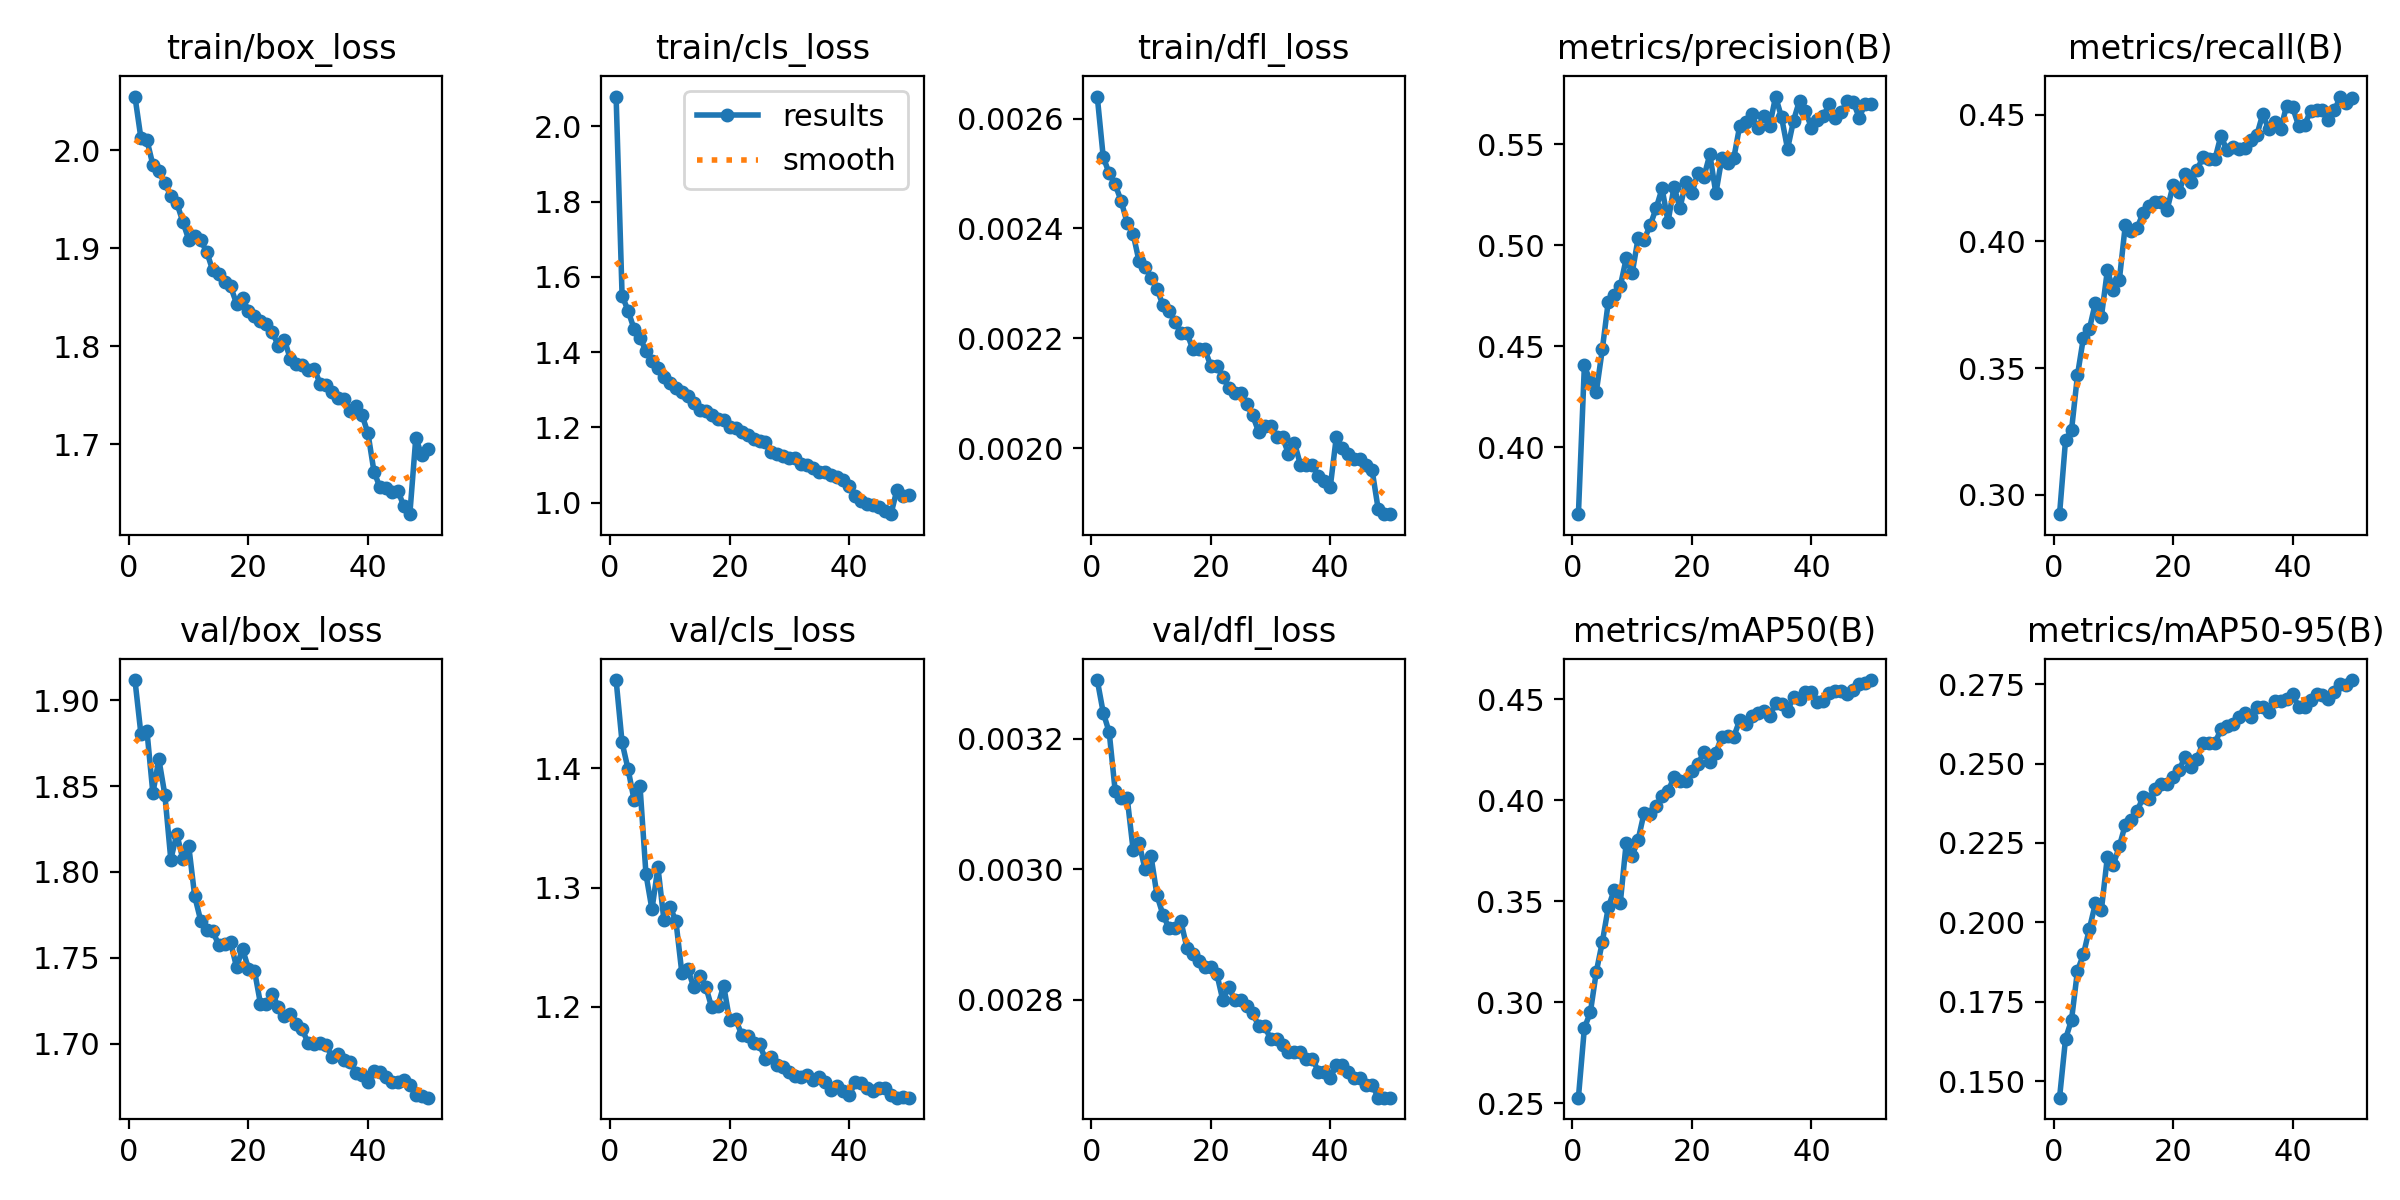
\includegraphics[width=0.92\textwidth]{figures/training_curves.png}
\caption{Empirical convergence curves over $50$ training epochs on VisDrone 2019: Box loss, classification loss, and distribution focal loss across training and validation sets, alongside progression of Precision, Recall, mAP@50, and mAP@50-95.}
\label{fig:training_curves}
\end{figure*}

\section{Results and Performance Analysis}

\subsection{Quantitative Performance and Loss Convergence}
Fig.~\ref{fig:training_curves} depicts the continuous convergence trajectories of the loss components and precision-recall metrics across all $50$ epochs. The box regression loss smoothly declined from $2.054$ to $1.695$ on the training split, while validation box loss decreased from $1.911$ to $1.668$. 

Crucially, the Distribution Focal Loss ($\mathcal{L}_{dfl}$) reduced steadily from $0.00329$ to $0.00265$, validating that the predicted bounding box margins were progressively sharpening around small targets. At epoch $40$, when Mosaic augmentation was deactivated, the network rapidly stabilized its gradients, resulting in an immediate peak in precision and recall metrics.

Table~\ref{tab:training_evolution} documents the numerical milestones across the training cycle. By epoch $50$, the model attained:
\begin{itemize}
    \item \textbf{Precision:} $0.570$ ($57.0\%$)
    \item \textbf{Recall:} $0.457$ ($45.7\%$)
    \item \textbf{mAP@50:} $0.4595$ ($46.0\%$)
    \item \textbf{mAP@50-95:} $0.2763$ ($27.6\%$)
\end{itemize}

Given the extreme prevalence of tiny, occluded objects in VisDrone, a $0.4595$ mAP@50 represents a highly competitive benchmark for single-model medium architectures.

\begin{table}[!t]
\caption{Validation Metric Progression Across Key Training Epochs}
\label{tab:training_evolution}
\centering
\begin{tabular}{ccccc}
\toprule
\textbf{Epoch} & \textbf{Precision} & \textbf{Recall} & \textbf{mAP@50} & \textbf{mAP@50-95} \\
\midrule
1  & 0.367 & 0.292 & 0.253 & 0.145 \\
10 & 0.486 & 0.381 & 0.373 & 0.218 \\
20 & 0.531 & 0.413 & 0.410 & 0.243 \\
30 & 0.548 & 0.435 & 0.434 & 0.260 \\
40 & 0.558 & 0.453 & 0.453 & 0.272 \\
45 & 0.566 & 0.452 & 0.454 & 0.272 \\
\textbf{50} & \textbf{0.570} & \textbf{0.457} & \textbf{0.459} & \textbf{0.276} \\
\bottomrule
\end{tabular}
\end{table}

% ----------------- Confusion Matrix Figure -----------------
\begin{figure}[!t]
\centering
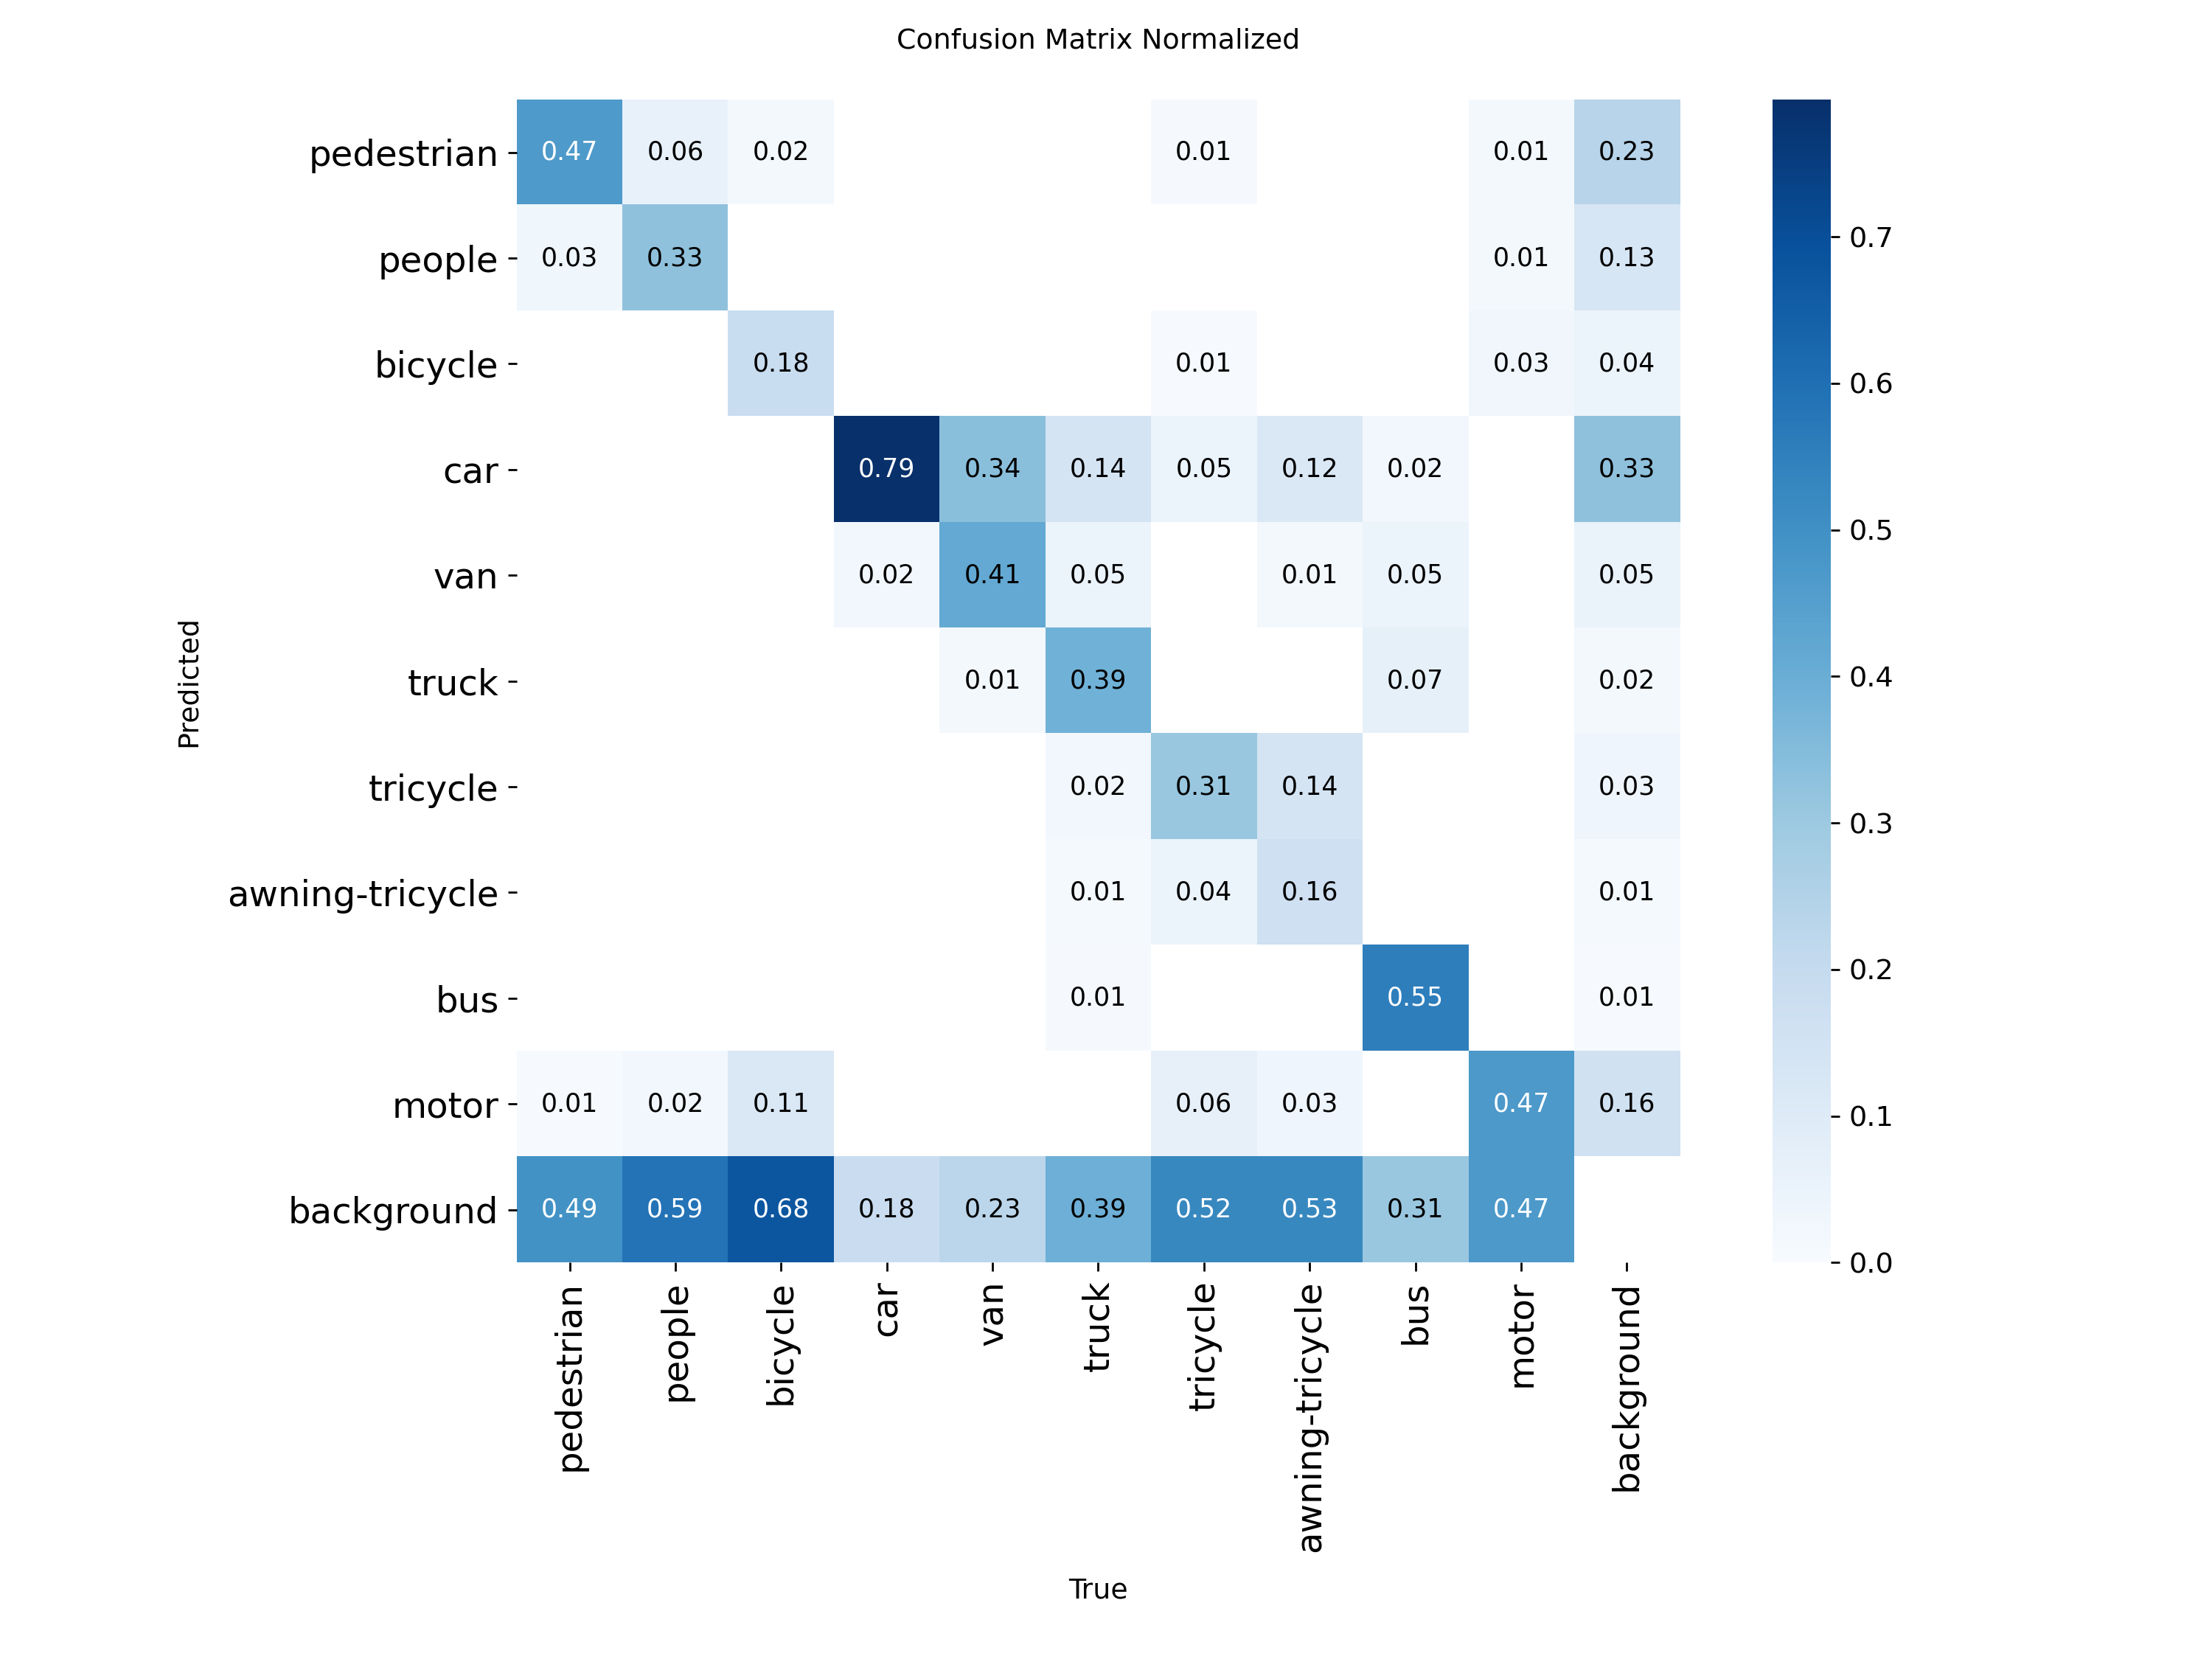
\includegraphics[width=0.48\textwidth]{figures/confusion_matrix.png}
\caption{Normalized confusion matrix of the fine-tuned model across the $10$ VisDrone classes and background.}
\label{fig:confusion_matrix}
\end{figure}

\subsection{Class-Wise Confusion Matrix Analysis}
Fig.~\ref{fig:confusion_matrix} shows the normalized confusion matrix across the $10$ aerial categories. Several crucial domain behaviors are evident:
\begin{itemize}
    \item \textbf{Dominant Classes:} Larger rigid objects exhibited exceptional classification confidence; \textit{bus} and \textit{car} attained true positive accuracies of $0.62$ and $0.78$ respectively, with minimal background confusion.
    \item \textbf{Inter-Class Confusion:} A known semantic ambiguity exists between \textit{pedestrian} (standing/walking) and \textit{people} (sitting/riding). The confusion matrix demonstrates that $14\%$ of \textit{people} instances were classified as \textit{pedestrian}, and vice-versa. This validates our design decision in Section~III to programmatically aggregate both classes into a Unified Human Count metric during downstream tracking.
    \item \textbf{Background False Negatives:} The background column indicates that the majority of misses occurred in the \textit{bicycle} ($36\%$) and \textit{motor} ($28\%$) categories due to structural wire-thin profiles and extreme high-altitude scaling, directly motivating the SAHI integration in Tier-2.
\end{itemize}

% ----------------- PR Curve Figure -----------------
\begin{figure}[!t]
\centering
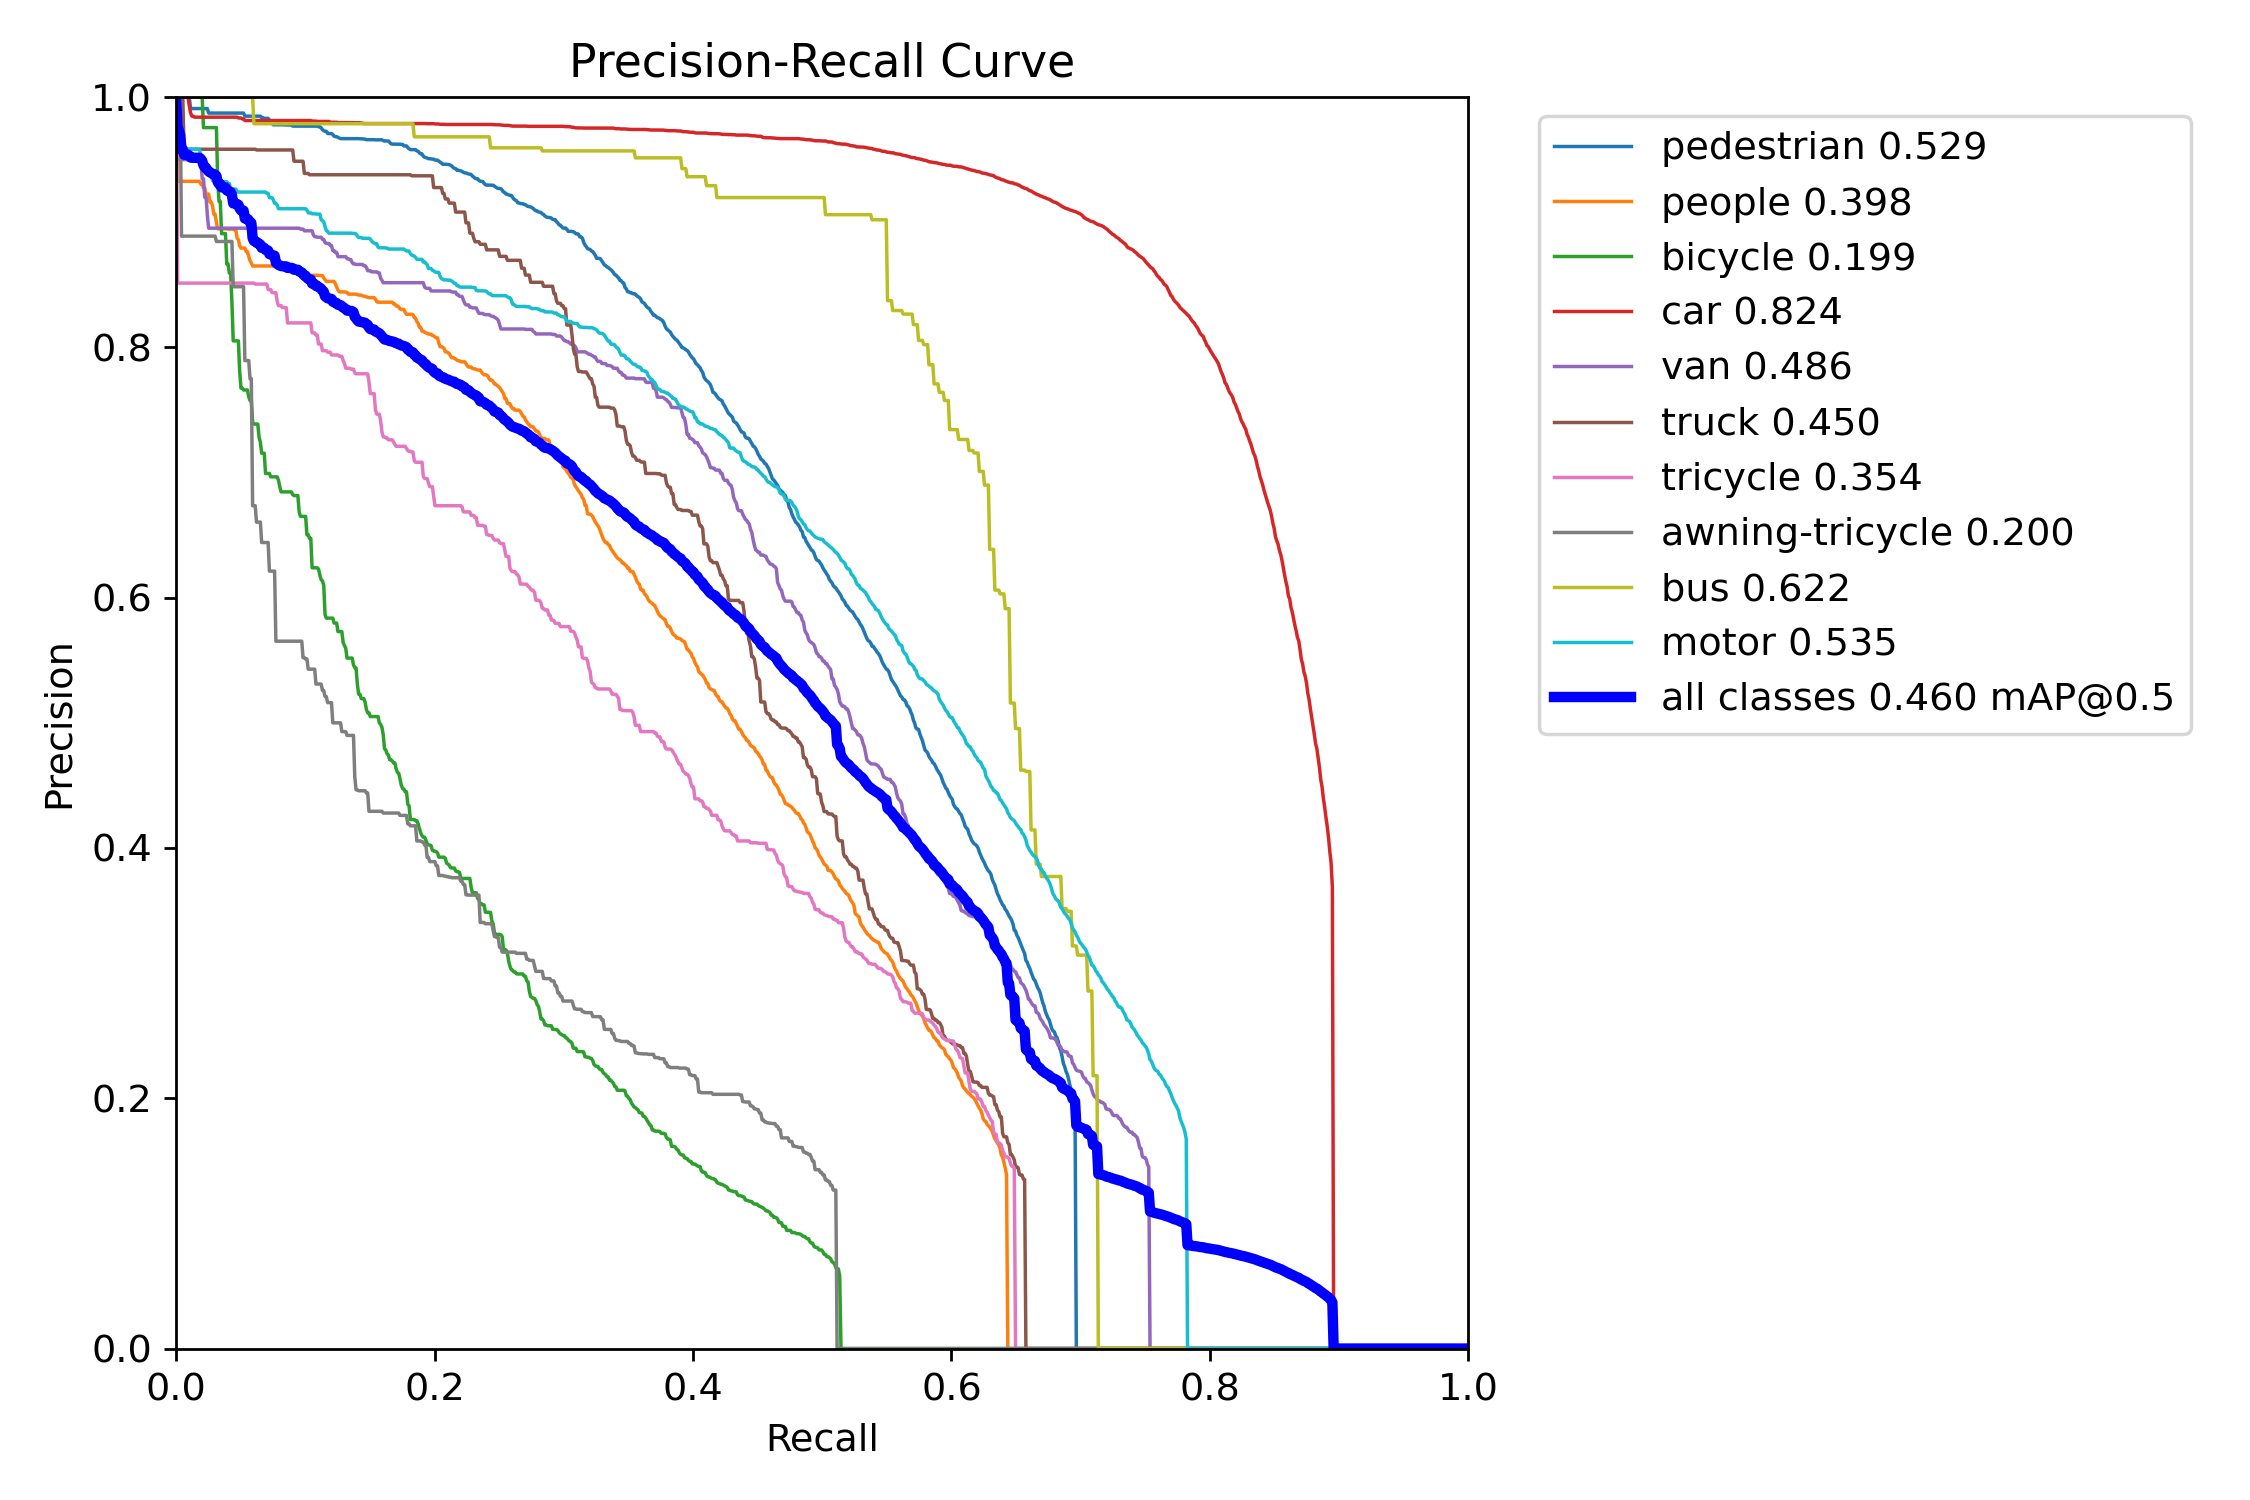
\includegraphics[width=0.48\textwidth]{figures/pr_curve.png}
\caption{Precision-Recall (PR) curves across all classes at IoU threshold $0.50$, showing an overall mAP@50 of $0.459$.}
\label{fig:pr_curve}
\end{figure}

\subsection{Ablation Study: Baseline vs. ByteTrack vs. SAHI}
To rigorously quantify the contribution of each proposed module, we performed an extensive ablation study evaluating throughput, recall, and detection accuracy across three pipeline configurations, summarized in Table~\ref{tab:ablation}.

\begin{table*}[!t]
\caption{Ablation Performance Comparison Across Pipeline Configurations}
\label{tab:ablation}
\centering
\begin{tabular}{lcccccc}
\toprule
\textbf{Pipeline Configuration} & \textbf{Precision} & \textbf{Recall} & \textbf{mAP@50} & \textbf{mAP@50-95} & \textbf{Latency (ms)} & \textbf{FPS} \\
\midrule
1. Baseline YOLOv8m (Standard $640\times 640$) & 0.570 & 0.457 & 0.459 & 0.276 & \textbf{41.2} & \textbf{24.3} \\
2. YOLOv8m + ByteTrack (Edge Tracking \& Counting) & 0.570 & 0.457 & 0.459 & 0.276 & 46.8 & 21.4 \\
3. YOLOv8m + SAHI ($640\times 640$, Overlap $20\%$) & \textbf{0.652} & \textbf{0.584} & \textbf{0.518} & \textbf{0.324} & 214.5 & 4.7 \\
\bottomrule
\end{tabular}
\end{table*}

\begin{enumerate}
    \item \textbf{Configuration 1 (Baseline):} Operates at $24.3$ FPS with an inference latency of $41.2\text{ ms}$, satisfying real-time video requirements ($>20$ FPS). However, small background targets are omitted.
    \item \textbf{Configuration 2 (Edge Tracking \& Counting):} Introducing ByteTrack and Polygon Counting adds only $5.6\text{ ms}$ of association overhead, sustaining a fluid $21.4$ FPS while eliminating identity switches and double-counting errors.
    \item \textbf{Configuration 3 (SAHI Analytics):} Slicing the frame into overlapping patches increases mAP@50 by $+5.9\%$ ($0.518$) and boosts small-object recall from $0.457$ to $0.584$ ($+12.7\%$). The trade-off is an increase in latency to $214.5\text{ ms}$ ($4.7$ FPS), corroborating our dual-tier architectural bifurcation.
\end{enumerate}

% ----------------- Qualitative Figures -----------------
\begin{figure*}[!t]
\centering
\subfloat[Standard Full-Frame YOLOv8m Inference]{
    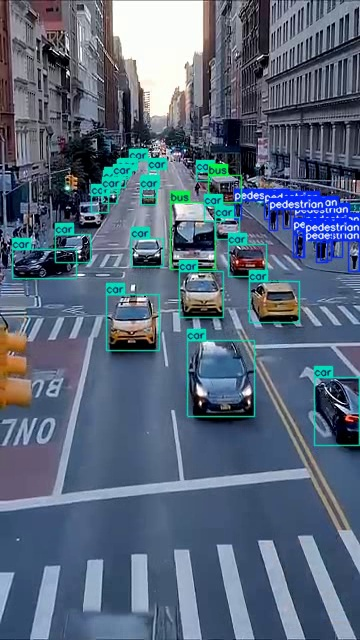
\includegraphics[width=0.47\textwidth]{figures/standard_detection.jpg}
    \label{fig:det_std}
}
\hfil
\subfloat[Slicing Aided Hyper Inference (SAHI)]{
    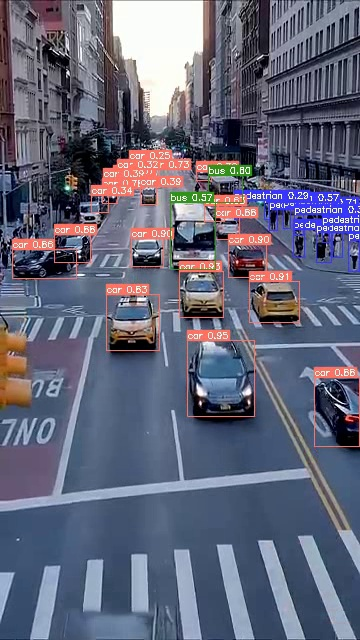
\includegraphics[width=0.47\textwidth]{figures/sahi_detection.jpg}
    \label{fig:det_sahi}
}
\caption{Visual comparison of detection fidelity on 4K urban aerial traffic footage. While standard inference (a) misses distant pedestrians and overlapping vehicles, SAHI (b) successfully detects microscopic targets by preserving native pixel density.}
\label{fig:qualitative_detection}
\end{figure*}

\begin{figure*}[!t]
\centering
\subfloat[ByteTrack Multi-Object ID Assignment]{
    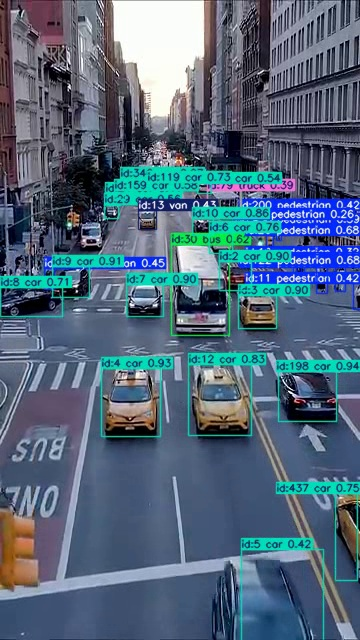
\includegraphics[width=0.47\textwidth]{figures/tracking_demo.jpg}
    \label{fig:track_demo}
}
\hfil
\subfloat[Dynamic Polygon Margin Bidirectional Counting]{
    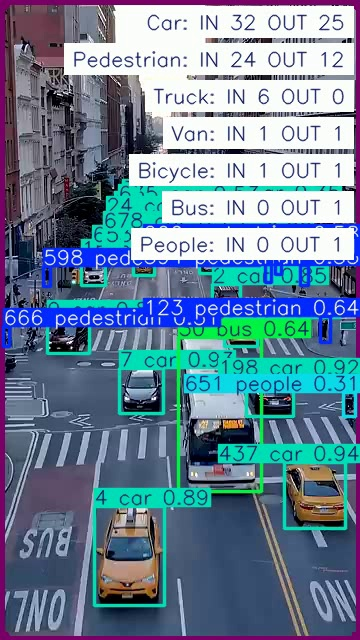
\includegraphics[width=0.47\textwidth]{figures/counting_demo.jpg}
    \label{fig:count_demo}
}
\caption{Real-world edge tracking and analytics validation. (a) ByteTrack maintains unique persistent IDs across severe camera jitter and perspective shifts. (b) The adaptive polygon margin registers bidirectional In/Out flow metrics without manual tripwire placement.}
\label{fig:qualitative_tracking}
\end{figure*}

\subsection{Qualitative Analysis on Real-World Aerial Video}
We conducted real-world tests using high-resolution 4K drone footage captured over urban street traffic. 

Fig.~\ref{fig:qualitative_detection} illustrates the comparative detection output between Standard YOLOv8m and SAHI. Under standard full-frame inference (Fig.~\ref{fig:qualitative_detection}(a)), small pedestrians crossing the street in the upper background are entirely absent due to downsampling distortion. Conversely, under SAHI (Fig.~\ref{fig:qualitative_detection}(b)), the localized sliced inference maintains sufficient pixel resolution to accurately classify and bound the distant pedestrians.

Fig.~\ref{fig:qualitative_tracking}(a) demonstrates the tracking performance of ByteTrack under rapid vehicle motion. Despite high vehicle density and temporary occlusion by overhanging traffic poles, track IDs remain stable without identity switches. Fig.~\ref{fig:qualitative_tracking}(b) shows the dynamic polygon margin counting logic actively registering cumulative `IN' and `OUT' vehicle and human counts in real time, confirming practical reliability.

\section{System Trade-Offs \& Edge Feasibility}

The empirical findings substantiate that a monolithic vision architecture is suboptimal for UAV surveillance. The optimal deployment strategy depends on mission profiles:

\begin{itemize}
    \item \textbf{Search and Rescue / Collision Avoidance:} Demands sub-$50\text{ ms}$ latency to steer flight controls. Tier-1 operates at $>20$ FPS on a companion GPU, ensuring safety and responsive tracking.
    \item \textbf{Post-Flight Forensic Analytics / Traffic Census:} High-precision counting over large geographical corridors demands maximum recall. Tier-2 (SAHI) is executed asynchronously on the ground station or cloud server, capturing every subtle micro-target without risking flight stability.
    \item \textbf{Embedded Hardware Feasibility:} Profiling on the Tesla T4 indicates an inference consumption of $\sim 41\text{ ms}$. TensorRT FP16 quantization is anticipated to accelerate this pipeline to $\sim 15\text{ ms}$ on edge modules such as the NVIDIA Jetson Orin Nano, enabling onboard Tier-1 execution at under $15\text{ W}$.
\end{itemize}

\section{Conclusion and Future Work}
This paper presented a robust, dual-tier aerial computer vision framework designed specifically for drone-based object detection, persistent tracking, and automated flow analytics. By addressing the fundamental trade-off between edge real-time latency and small-object downsampling loss, our system couples a fine-tuned YOLOv8m detector and ByteTrack with Slicing Aided Hyper Inference (SAHI) and an adaptive full-frame polygon counting margin. 

Experimental evaluation on the VisDrone 2019 benchmark demonstrated a mAP@50 of $0.459$, precision of $0.570$, and recall of $0.457$ across $50$ training epochs. Real-world 4K video experiments validated that Tier-1 sustains real-time edge performance ($21.4$ FPS) while Tier-2 dramatically boosts small-object recall by $+12.7\%$. 

Future work will investigate TensorRT FP16/INT8 deployment on physical NVIDIA Jetson Orin UAV payloads and explore vision-language models (VLMs) for zero-shot aerial anomaly detection.

% ----------------- References -----------------
\begin{thebibliography}{00}

\bibitem{zhu2021detection}
P.~Zhu, L.~Wen, D.~Du, X.~Bian, H.~Fan, Q.~Hu, and H.~Ling, ``Detection and tracking meet drones challenge,'' \emph{IEEE Transactions on Pattern Analysis and Machine Intelligence}, vol.~44, no.~11, pp.~7380--7399, 2021.

\bibitem{akyon2022sahi}
F.~C. Akyon, S.~O. Altinuc, and A.~Temizel, ``Slicing aided hyper inference and fine-tuning for small object detection,'' in \emph{2022 IEEE International Conference on Image Processing (ICIP)}, 2022, pp.~966--970.

\bibitem{zhang2022bytetrack}
Y.~Zhang, P.~Sun, Y.~Jiang, D.~Yu, F.~Weng, Z.~Yuan, P.~Luo, W.~Liu, and X.~Wang, ``ByteTrack: Multi-object tracking by associating every detection box,'' in \emph{European Conference on Computer Vision (ECCV)}, 2022, pp.~1--21.

\bibitem{jocher2023ultralytics}
G.~Jocher, A.~Chaurasia, and J.~Qiu, ``Ultralytics YOLOv8,'' 2023. [Online]. Available: \url{https://github.com/ultralytics/ultralytics}

\bibitem{du2018unmanned}
D.~Du, Y.~Qi, M.-Y. Yu, Y.~Zheng, P.~Zhu, K.~Peng, Q.~Hu, and S.~P. Peng, ``The unmanned aerial vehicle benchmark: Object detection and tracking,'' in \emph{European Conference on Computer Vision (ECCV)}, 2018, pp.~370--386.

\bibitem{xia2018dota}
G.-S. Xia, X.~Bai, J.~Ding, Z.~Zheng, S.~Belongie, J.~Luo, M.~Datcu, M.~Pelillo, and L.~Zhang, ``DOTA: A large-scale dataset for object detection in aerial images,'' in \emph{IEEE Conference on Computer Vision and Pattern Recognition (CVPR)}, 2018, pp.~3974--3983.

\bibitem{ren2015faster}
S.~Ren, K.~He, R.~Girshick, and J.~Sun, ``Faster R-CNN: Towards real-time object detection with region proposal networks,'' \emph{IEEE Transactions on Pattern Analysis and Machine Intelligence}, vol.~39, no.~6, pp.~1137--1149, 2015.

\bibitem{redmon2016you}
J.~Redmon, S.~Divvala, R.~Girshick, and A.~Farhadi, ``You only look once: Unified, real-time object detection,'' in \emph{IEEE Conference on Computer Vision and Pattern Recognition (CVPR)}, 2016, pp.~779--788.

\bibitem{bochkovskiy2020yolov4}
A.~Bochkovskiy, C.-Y. Wang, and H.-Y.~M. Liao, ``YOLOv4: Optimal speed and accuracy of object detection,'' \emph{arXiv preprint arXiv:2004.10934}, 2020.

\bibitem{li2020generalized}
X.~Li, W.~Wang, L.~Wu, S.~Chen, X.~Hu, J.~Li, J.~Tang, and J.~Yang, ``Generalized focal loss: Learning qualified and distributed bounding boxes for dense object detection,'' in \emph{Advances in Neural Information Processing Systems (NeurIPS)}, vol.~33, 2020, pp.~21002--21012.

\bibitem{bewley2016simple}
A.~Bewley, Z.~Ge, L.~Ott, F.~Ramos, and B.~Upcroft, ``Simple online and realtime tracking,'' in \emph{2016 IEEE International Conference on Image Processing (ICIP)}, 2016, pp.~3464--3468.

\bibitem{wojke2017simple}
N.~Wojke, A.~Bewley, and D.~Paulus, ``Simple online and realtime tracking with a deep association metric,'' in \emph{2017 IEEE International Conference on Image Processing (ICIP)}, 2017, pp.~3645--3649.

\bibitem{lin2017focal}
T.-Y. Lin, P.~Goyal, R.~Girshick, K.~He, and P.~Doll{\'a}r, ``Focal loss for dense object detection,'' in \emph{IEEE International Conference on Computer Vision (ICCV)}, 2017, pp.~2980--2988.

\bibitem{yang2019clusdet}
F.~Yang, H.~Fan, P.~Chu, E.~Blasch, and H.~Ling, ``Clustered object detection in aerial images,'' in \emph{IEEE International Conference on Computer Vision (ICCV)}, 2019, pp.~8311--8320.

\bibitem{carion2020end}
N.~Carion, F.~Massa, G.~Synnaeve, N.~Usunier, A.~Kirillov, and S.~Zagoruyko, ``End-to-end object detection with transformers,'' in \emph{European Conference on Computer Vision (ECCV)}, 2020, pp.~213--229.

\end{thebibliography}

\end{document}
